\documentclass{beamer}
\newcommand{\fttheory}[1]{\fcolorbox{blue}{blue}{\color{white}\textbf{#1}\hspace{\textwidth}}}
\newcommand{\ftexampl}[1]{\fcolorbox{orange}{orange}{\color{black}\textbf{#1}\hspace{\textwidth}}}
\newcommand{\ftdata}[1]{\fcolorbox{violet}{violet}{\color{white}\textbf{#1}\hspace{\textwidth}}}
\newcommand{\ftheader}[1]{\fcolorbox{lightgray}{lightgray}{\color{black}\textbf{#1}\hspace{\textwidth}}}
\begin{document}

\begin{frame}{\ftheader{Capital Asset Pricing Model.}}
\begin{itemize}
\item The capital asset pricing model (CAPM) is used to determine a theoretically appropriate required rate of return of an asset, {if that asset is to be added to an already well-diversified portfolio (market portfolio)}.
\item The model takes into account the {asset's sensitivity to market risk} (also known as systematic risk or non-diversifiable risk), often represented by the quantity beta ($\beta$) in the financial industry, as well as the expected return of the market and the expected return of a theoretical risk-free asset. 
\end{itemize}
\end{frame}

% Independent Risk
\begin{frame}{\fttheory{The Market Portfolio}}
	\begin{itemize}
		\item In our last lecture, we constructed an efficient frontier, capital allocation lines, and the tangency portfolio using two stocks and the risk-free asset
		\item Suppose that we repeated the exercise with \underline{all} securities, not just two. We would obtain a tangency portfolio, a capital allocation line (known as the security market line (SML)) 
		\item The market portfolio is the value-weighted portfolio of \underline{all} securities (yes, \underline{all} of them)...
		\item ...but in practice, we approximate the returns of the market portfolio with the returns of the S\&P 500
		\item Investors \underline{demand} a combination of the risk-free asset and the tangency portfolio; the market \underline{supplies} the market portfolio and the risk-free asset
		\item In equilibrium, demand equals supply: 
	\end{itemize}
	\begin{center}
		The tangency portfolio of all securities equals the market portfolio 
	\end{center}
\end{frame}

% Independent Risk
\begin{frame}{\fttheory{Systematic and Idiosyncratic Risks}}
	\noindent\textbf{Systematic Risk}
	\begin{itemize}
		\item Systematic risk is risk to which \underline{all} firms are exposed
		\item Apple examples: sales fall when unemployment rises, wages fall; conversely, sales rise when unemployment falls, wages rise
		\item Home Depot is exposed to the same risks
	\end{itemize}
	\noindent\textbf{Idiosyncratic Risk}
	\begin{itemize}
		\item Idiosyncratic risk is risk specific to the firm
		\item Apple examples: problems with Foxconn (an Apple supplier), Steve Jobs dies, the Justice Department figures out how to hack iPhones, etc.
		\item Home Depot is not exposed (directly) to these risks
	\end{itemize}
\end{frame}


% A Preview of the CAPM 
\begin{frame}{\fttheory{The CAPM in a Nutshell}}
\begin{itemize}
\item In a nutshell, the CAPM says that
\begin{equation*}
\overbrace{R_{\text{Stock}}-R_{F}}^{\text{Stock Return}}=\overbrace{\beta_{\text{Stock}}\times(R_{\text{Market}}-R_{F})}^{\text{Systematic Risk}}+\overbrace{\epsilon_{\text{Stock}}}^{\text{Idiosyncratic Risk}}
\end{equation*}
where $\epsilon_{\text{Stock}}$ is a random shock to the stock's return 
\item \textbf{Important:} $\text{E}[\epsilon_{\text{Stock}}]=0$ and $\text{Cov}[R_{\text{Market}},\epsilon_{\text{Stock}}]=0$
\item Taking expectations, 
\begin{equation*}
\overbrace{E[R_{\text{Stock}}]-R_{F}}^{\text{Stock Risk Premium}}=\beta_{\text{Stock}}\times\overbrace{(E[R_{\text{Market}}]-R_{F})}^{\text{Equity Risk Premium}}
\end{equation*}
\item Investors are \underline{not} compensated for idiosyncratic risk: the stock's risk premium only depends on its beta ($\beta_{\text{Stock}}$) and the equity risk premium (a.k.a. market risk premium)
\end{itemize}
\end{frame}

% Sensitivity to Systematic Risk: Beta
\begin{frame}{\fttheory{Beta}}
\begin{equation*}
\overbrace{R_{\text{Stock}}-R_{F}}^{\text{Stock Return}}=\overbrace{\beta_{\text{Stock}}\times(R_{\text{Market}}-R_{F})}^{\text{Systematic Risk}}+\overbrace{\epsilon_{\text{Stock}}}^{\text{Idiosyncratic Risk}}
\end{equation*}
\begin{itemize}
\item $\beta_{\text{Stock}}$ (Beta) is the slope of the regression line obtained by regressing the stock's returns on the market's returns
\begin{equation}
\beta_{\text{Stock}}=\frac{\text{Cov}[R_{\text{Stock}},R_{\text{Market}}]}{\text{Var}[R_{\text{Market}}]}
\end{equation}
\item The beta of a security is the expected \% change in its return given a 1\% change in the return of the market portfolio
\item It is the sensitivity of the stock's returns to systematic risk
\end{itemize}
\end{frame}

%%%%%%%%%%%%%%%%%%  SLIDE  %%%%%%%%%%%%%%%%%%
\begin{frame}{\ftdata{CAPM Beta: Examples}}
	\begin{center}
		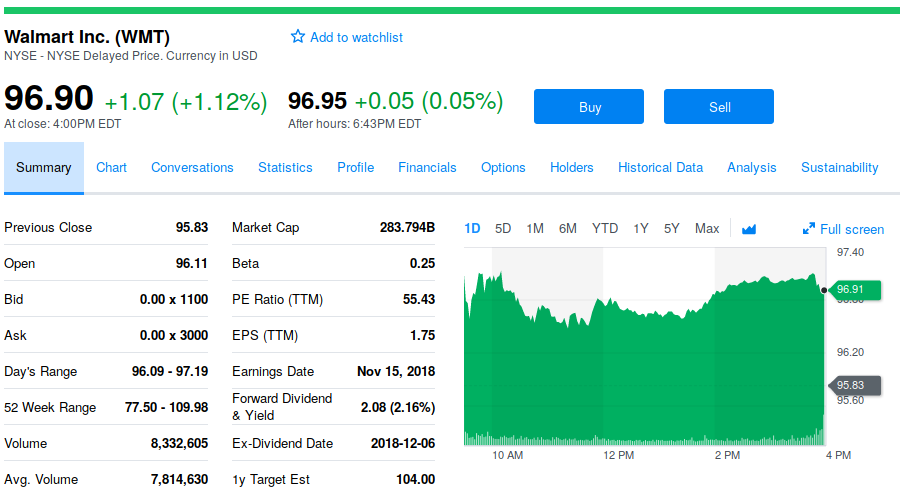
\includegraphics[scale=0.35]{wmt.png}
	\end{center}
	\begin{center}
		Walmart has a beta of \textbf{0.25}
	\end{center}
\end{frame}

%%%%%%%%%%%%%%%%%%  SLIDE  %%%%%%%%%%%%%%%%%%
\begin{frame}{\ftdata{CAPM Beta: Examples}}
	\begin{center}
		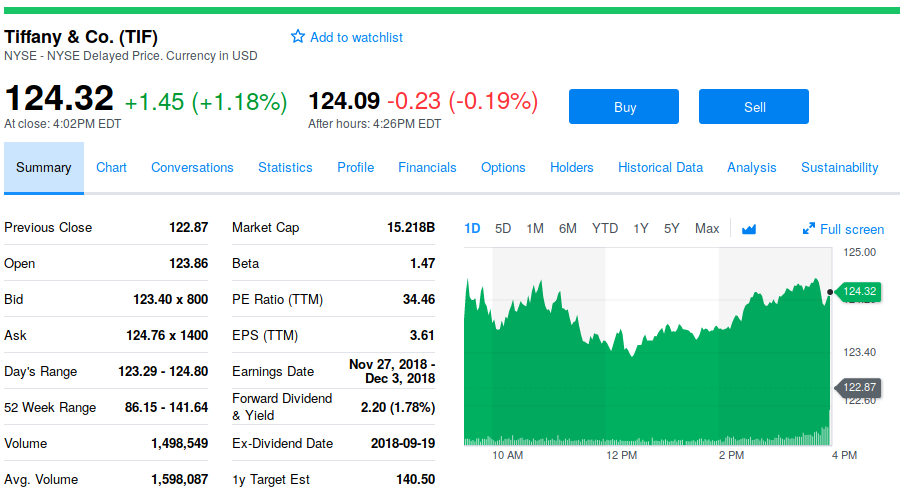
\includegraphics[scale=0.35]{tif.png}
	\end{center}
	\begin{center}
		Tiffany's has a beta of \textbf{1.47}
	\end{center}
\end{frame}

% Variance Decomposition
\begin{frame}{\fttheory{Volaility Decomposition}}
\begin{itemize}
\item The stock's volatility is $\text{SD}[R_{\text{Stock}}]$ 
\item The volatility of a porfolio with the same systematic risk as that of the stock is $\beta_{\text{Stock}}\text{SD}[R_{\text{Market}}]$
\item We say that a fraction 
	\begin{equation}\label{eq:systematic}
		\frac{\beta_{\text{Stock}}\text{SD}[R_{\text{Market}}]}{\text{SD}[R_{\text{Stock}}]}
	\end{equation}
of the stock's volatility is systematic; we say that the remaining fraction is idiosyncratic
\item Note that Equation \ref{eq:systematic} is just $\sqrt{R^{2}}$ from regression analysis
\end{itemize}
\end{frame}

% Example
\begin{frame}{\ftexampl{Example}}
	Consider the following data for Cisco (CSCO) and the market
	\begin{center}
		\begin{tabular}{ll}
			$\text{E}[R_{\text{CSCO}}]=0.9961\%$ & $\text{SD}[R_{\text{CSCO}}]=7.09\%$ \\
			$\text{E}[R_{\text{MKT}}]=1.0773\%$ & $\text{SD}[R_{\text{MKT}}]=3.7568\%$ \\
			$\text{Corr}[R_{\text{CSCO}},R_{\text{MKT}}]=0.6339$ & $R_{F}=0.0418\%$
		\end{tabular}
	\end{center}
\begin{enumerate}
	\item What are Cisco's and the market's Sharpe ratios? {\color{blue} .1346, .2756} 
	\item What is Cisco's beta? {\color{blue}1.1963}
	\item What is the market's risk premium? {\color{blue}1.0355\%}
	\item What is Cisco's risk premium? {\color{blue}0.9543\%}
	\item What fraction of Cisco's volatility is systematic? {\color{blue} .6339}
	\item What fraction is idiosyncratic? {\color{blue} .3661}
\end{enumerate}
\end{frame}

% Example
\begin{frame}{\ftexampl{Example}}
	Consider the following data for Caterpillar (CAT) and the market
	\begin{center}
		\begin{tabular}{ll}
			$\text{E}[R_{\text{CAT}}]=1.3424\%$ & $\text{SD}[R_{\text{CAT}}]=8.1365\%$ \\
			$\text{E}[R_{\text{MKT}}]=1.0773\%$ & $\text{SD}[R_{\text{MKT}}]=3.7568\%$ \\
			$\text{Corr}[R_{\text{CAT}},R_{\text{MKT}}]=0.7279$ & $R_{F}=0.0418\%$
		\end{tabular}
	\end{center}
\begin{enumerate}
	\item What are Caterpillar's and the market's Sharpe ratios? 
	\item What is Caterpillar's beta 
	\item What is the market's risk premium? 
	\item What is Caterpillar's risk premium? 
	\item What fraction of Caterpillar's volatility is systematic? 
	\item What fraction is idiosyncratic?
\end{enumerate}
\end{frame}

\begin{frame}{\fttheory{Alpha}}
	\begin{itemize}
	\item The difference between the stock's actual risk premium and the risk premium of a portfolio with the same systematic risk is the alpha:  
	\begin{equation}
		\alpha_{\text{Stock}} = \underbrace{(\text{E}[R_{\text{Stock}}]-R_{F})}_{\text{True Value}}-\underbrace{\beta_{\text{Stock}}\times(\text{E}[R_{\text{Market}}] - R_{F})}_{\text{CAPM}}
	\end{equation}
	\item If $\alpha\neq0$, then one can make an arbitrage profit 
	\begin{itemize}
	\item If $\alpha>0$, then go long 
	\item If $\alpha<0$, then go short 
	\end{itemize}
	\item While one might observe a non-zero alpha in the short-term, it will likely become zero in the long-term
	\end{itemize}
\end{frame}

% Example
\begin{frame}{\ftexampl{Example}}
\begin{enumerate}
	\item What is Cisco's alpha? {\color{blue}-0.2845\%}
	\item Should we go long or short? {\color{blue}short}
	\item What about Caterpillar?
\end{enumerate}
\end{frame}

\end{document}
